%%%%%%%%%%%%%%%%%%%%%%%%%%%%%%%%%%%%%%%%%
% Short Sectioned Assignment
% LaTeX Template
% Version 1.0 (5/5/12)
%
% This template has been downloaded from:
% http://www.LaTeXTemplates.com
%
% Original author:
% Frits Wenneker (http://www.howtotex.com)
%
% License:
% CC BY-NC-SA 3.0 (http://creativecommons.org/licenses/by-nc-sa/3.0/)
%
%%%%%%%%%%%%%%%%%%%%%%%%%%%%%%%%%%%%%%%%%

%----------------------------------------------------------------------------------------
%	PACKAGES AND OTHER DOCUMENT CONFIGURATIONS
%----------------------------------------------------------------------------------------

\documentclass[paper=a4, fontsize=11pt]{scrartcl} % A4 paper and 11pt font size

\usepackage[utf8]{inputenc}
%\usepackage[T1]{fontenc} % Use 8-bit encoding that has 256 glyphs
\usepackage{fourier} % Use the Adobe Utopia font for the document - comment this line to return to the LaTeX default
\usepackage[english]{babel} % English language/hyphenation
\usepackage{amsmath,amsfonts,amsthm} % Math packages

\usepackage{nameref}
\usepackage{graphicx} % Required to insert images
%\usepackage{lipsum} % Used for inserting dummy 'Lorem ipsum' text into the template

\usepackage{sectsty} % Allows customizing section commands
\allsectionsfont{\centering \normalfont\scshape} % Make all sections centered, the default font and small caps

\usepackage{fancyhdr} % Custom headers and footers
\pagestyle{fancyplain} % Makes all pages in the document conform to the custom headers and footers
\fancyhead{} % No page header - if you want one, create it in the same way as the footers below
\fancyfoot[L]{} % Empty left footer
\fancyfoot[C]{} % Empty center footer
\fancyfoot[R]{\thepage} % Page numbering for right footer
\renewcommand{\headrulewidth}{0pt} % Remove header underlines
\renewcommand{\footrulewidth}{0pt} % Remove footer underlines
\setlength{\headheight}{13.6pt} % Customize the height of the header

%\numberwithin{equation}{section} % Number equations within sections (i.e. 1.1, 1.2, 2.1, 2.2 instead of 1, 2, 3, 4)
%\numberwithin{figure}{section} % Number figures within sections (i.e. 1.1, 1.2, 2.1, 2.2 instead of 1, 2, 3, 4)
%\numberwithin{table}{section} % Number tables within sections (i.e. 1.1, 1.2, 2.1, 2.2 instead of 1, 2, 3, 4)

\setlength\parindent{0pt} % Removes all indentation from paragraphs - comment this line for an assignment with lots of text

%----------------------------------------------------------------------------------------
%	TITLE SECTION
%----------------------------------------------------------------------------------------

\newcommand{\horrule}[1]{\rule{\linewidth}{#1}} % Create horizontal rule command with 1 argument of height

\title{	
\normalfont \normalsize 
\textsc{Università della Svizzera Italiana, Faculty of Informatics} \\ [25pt] % Your university, school and/or department name(s)
\horrule{0.5pt} \\[0.4cm] % Thin top horizontal rule
\huge Filtering Noisy Data \\ % The assignment title
\horrule{2pt} \\[0.5cm] % Thick bottom horizontal rule
}

\author{Simon Maurer} % Your name

\date{\normalsize\today} % Today's date or a custom date

\begin{document}

\maketitle % Print the title

%----------------------------------------------------------------------------------------
%	PROBLEM 1
%----------------------------------------------------------------------------------------

\section{Assignment 3.1}

The mean vector $ \boldsymbol{\mu} = [x_1, x_2]^T $ can be calculated with:
\begin{equation}
    x_k = \frac{1}{N}\sum\limits_{i=1}^{N} x_{ki}
\end{equation}
Using the given input data, we get $ \boldsymbol{\mu} = [5.02, 10.03]^T $. The
vector is represented as a red dot in figure \ref{fig:dist}.

The covariance matrix can be calculated by using the command $ cov $ in
Octave\footnote{https://www.gnu.org/software/octave} or manually  by the
following equations:
\begin{equation}
    \Sigma = \begin{bmatrix}
        q_{11} & q_{12} \\
        q_{21} & q_{22}
    \end{bmatrix}
\end{equation}
where
\begin{equation}
    q_{ij} = \frac{1}{N-1} \sum\limits_{k=1}^{N} (x_{ik} - x_i)(x_{jk} - x_j)
\end{equation}
Using the given input data, we get $ \Sigma = 
\begin{bmatrix}
    1.05 & 0.58 \\
    0.58 & 2.06
\end{bmatrix} $

With the command $ inv $ and $ det $ in Octave, we calculate the inverse and
the determinant of the covariance matrix: $ \Sigma^{-1} =
\begin{bmatrix}
    1.13 & -0.32 \\
    -0.32 & 0.58
\end{bmatrix} $ and $ |\Sigma| = 1.82 $.

To calculate the blue vectors represented on figure \ref{fig:dist}, we can use
the command $ eig $ in Octave and get the eigenvectors and the eigenvalues of
the covariance matrix. The eigenvectors indicate the respective direction of
the vectors and the square root of the eigenvalue corresponds to their
respective length.

\begin{figure}[h]
    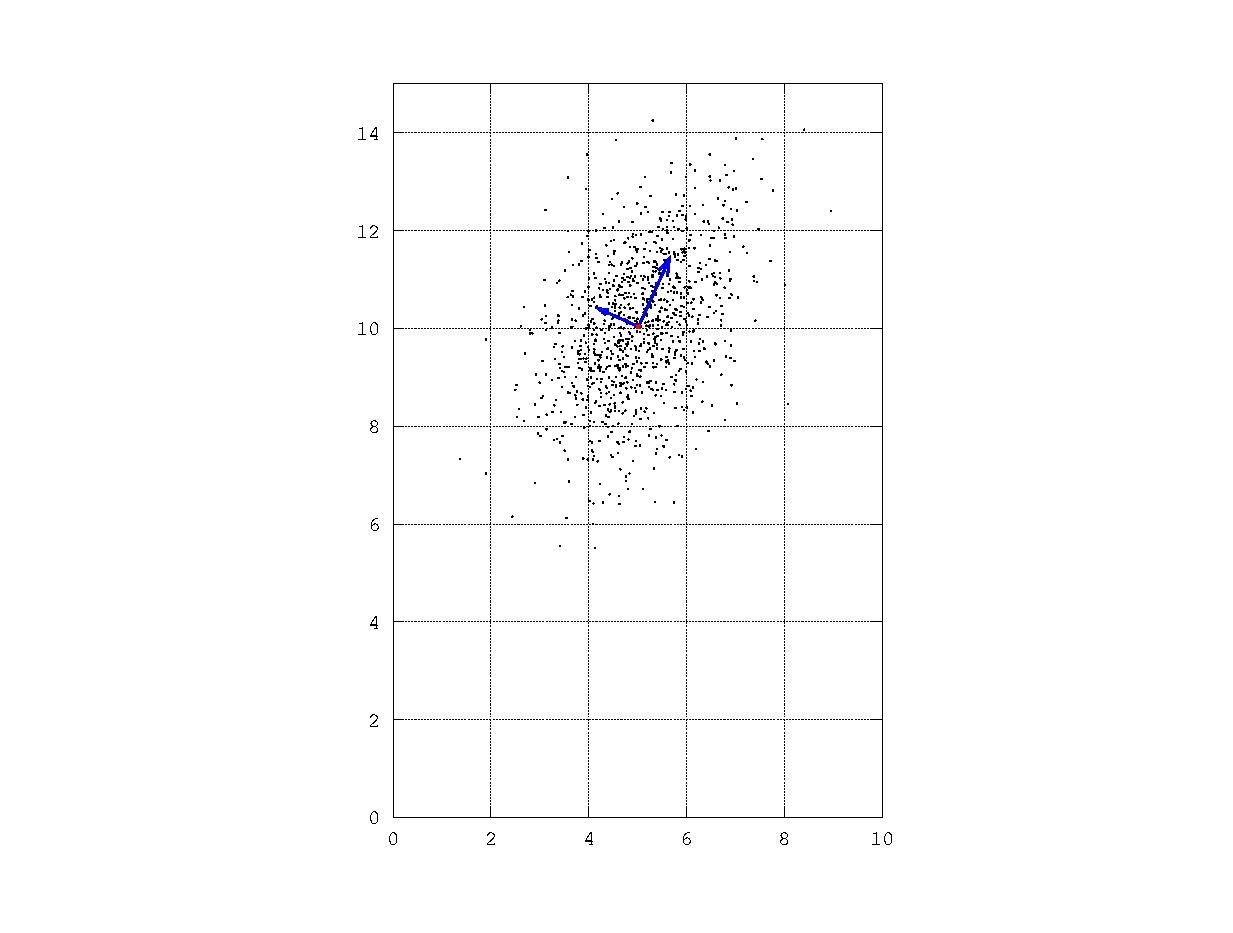
\includegraphics[width=1\columnwidth]{ex03_graph}
    \caption{Multivariate normal distribution with mean and standard deviation
        vectors}\label{fig:dist}
\end{figure}
\end{document}
